\documentclass[twoside,11pt]{article}

% Any additional packages needed should be included after jmlr2e.
% Note that jmlr2e.sty includes epsfig, amssymb, natbib and graphicx,
% and defines many common macros, such as 'proof' and 'example'.
%
% It also sets the bibliographystyle to plainnat; for more information on
% natbib citation styles, see the natbib documentation, a copy of which
% is archived at http://www.jmlr.org/format/natbib.pdf

\usepackage{jmlr2e}
\usepackage{amsmath}
\usepackage{amsfonts}
\usepackage{amssymb}
\usepackage{mathptmx}
\usepackage{hyperref}
\usepackage{dsfont}
\usepackage{algorithm}
\usepackage{algorithmicx}
\usepackage{algpseudocode}
\usepackage{subfigure}
\newtheorem{claim}{Claim}
% Definitions of handy macros can go here

%\newcommand{\dataset}{{\cal D}}
%\newcommand{\fracpartial}[2]{\frac{\partial #1}{\partial  #2}}

% Heading arguments are {volume}{year}{pages}{submitted}{published}{author-full-names}
\usepackage{lastpage}
\jmlrheading{19}{2018}{1-\pageref{LastPage}}{3/17; Revised
12/17}{11/18}{17-128}{Karl Rohe, Jun Tao, Xintian Han, and Norbert Binkiewicz}
%\jmlrheading{19}{2018}{1-13}{3/17}{00/00}{17-128}{Karl Rohe, Jun Tao, Xintian Han, and Norbert Binkiewicz}

% Short headings should be running head and authors last names

\ShortHeadings{Quickly Sampling a Sparse Matrix with Low Rank Expectation}{Rohe, Tao, Han, and  Binkiewicz}
\firstpageno{1}

\begin{document}

\title{A Note on Quickly Sampling a Sparse Matrix with Low Rank Expectation}

\author{\name Karl Rohe \email   karlrohe@stat.wisc.edu\\
       \addr Statistics Department \\
       University of Wisconsin-Madison\\
       Madison, WI 53706, USA
       \AND
       \name Jun Tao \email iTaojun@pku.edu.cn \\
       \addr School of Mathematical Sciences\\
            Peking University\\
       Beijing, 100871, China
        \AND
       \name Xintian Han \email hanxintian@pku.edu.cn \\
       \addr Yuanpei College\\
       Peking University\\
       Beijing, 100871, China
       \AND
       \name Norbert Binkiewicz \email norbertbin@gmail.com\\
        \addr Statistics Department \\
       University of Wisconsin-Madison\\
       Madison, WI 53706, USA
       }
       

\editor{Inderjit Dhillon}

\maketitle


\begin{abstract}%   <- trailing '%' for backward compatibility of .sty file
Given matrices $X,Y \in \mathds{R}^{n \times K}$ and $S \in \mathds{R}^{K \times K}$ with positive elements, this paper proposes an algorithm \texttt{fastRG} to sample a sparse matrix $A$ with low rank expectation $E(A) = XSY^T$ and independent Poisson elements.  This allows for quickly sampling from a broad class of stochastic blockmodel graphs (degree-corrected, mixed membership, overlapping) all of which are specific parameterizations of the generalized random product graph model defined in Section \ref{gRPG}. The basic idea of \texttt{fastRG} is to first sample the number of edges $m$ and then sample each edge. The key insight is that because of the the low rank expectation, it is easy to sample individual edges.  The naive ``element-wise'' algorithm requires $O(n^2)$ operations to generate the $n\times n$ adjacency matrix $A$.  In sparse graphs, where $m = O(n)$, ignoring log terms, \texttt{fastRG} runs in time $O(n)$.  An implementation in \texttt{R} is available on github.  A computational experiment in Section \ref{sec:implementation} simulates graphs up to $n=10,000,000$ nodes with $m = 100,000,000$ edges.  For example, on a graph with $n=500,000$ and $m = 5,000,000$, \texttt{fastRG} runs in less than one second on a 3.5 GHz Intel i5.  
%Moreover, \texttt{fastRG} could be easily parallelized.  
%Such network models serve as test beds of various types of clustering and statistical inference algorithms.  In performing simulation experiments, many of these statistical algorithms run dramatically faster than the time to simulate a single network. This note seeks to remove the bottleneck in such simulations by providing a simple linear time algorithm to sample from the RDPG. 
\end{abstract}

\begin{keywords}
Random Dot Product Graph, Edge exchangeable, Simulation

\end{keywords}

\section{Introduction}
The random dot product graph (RDPG) model serves as a test bed for various types of clustering and statistical inference algorithms. 
This model generalizes the Stochastic Blockmodel (SBM), the Overlapping SBM, the Mixed Membership SBM, and the Degree-Corrected SBM \citep{Holland1983Stochastic,
Latouche2011Overlapping,
Airoldi2008Mixed,
PhysRevE.83.016107}. Under the RDPG, each node $i$ has a (latent) node feature $x_i\in \mathds{R}^K$ and the probability that node $i$ and $j$ share an edge is parameterized by $\langle x_i , x_j \rangle$ \citep{Young2007}. 

While many network analysis algorithms only require $O(m)$ operations, where $m$ is the number of edges in the graph, sampling RDPGs with the naive ``element-wise'' algorithm takes  $O(n^2)$ operations, where $n$ is the number of nodes.  In particular, sparse eigensolvers compute the leading $k$ eigenvectors of such graphs in $O(km)$ operations (e.g. in ARPACK \citealt{lehoucqarpack}).  As such, sampling an RDPG is a computational bottleneck in simulations to examine many network analysis algorithms.
%Recently proven results give a central limit theorem for these eigenvectors under the Bernoulli RDPG \citep{athreya2016limit, tang2016limit}. 

%This paper introduces a slight generalization of the RDPG model (gRPG) and then presents a simple algorithm \texttt{fastRG} for sampling a gRPG in $O(m)$ operations.  In sparse graphs, $O(m) = O(n)$, and the speed advantages of \texttt{fastRG} are pronounced. Our simulation is exact in a multi-edge graph where the number of edges between $i$ and $j$ is $Poisson(\langle x_i,x_j\rangle)$; for example, the Degree Corrected SBM was originally proposed to have Poisson multi-edges \citep{PhysRevE.83.016107}. \texttt{fastRG} is a generalization of the sampling algorithm proposed in \cite{PhysRevE.83.016107}. Section \ref{gRPG} proposes the gRPG. 

The organization of this paper is as follows.  Section \ref{fastRG} gives \texttt{fastRG}. Section \ref{sec:xlr} relates \texttt{fastRG} to xlr, a new class of edge-exchangeable random graphs with low-rank expectation.  Section \ref{gRPG} presents a generalization of the random dot product graph. Theorem \ref{theoremRDPG} shows that \texttt{fastRG} samples Poisson-edge graphs from this model.  Then, Theorem \ref{theoremThresh} in Section \ref{approximate} shows how \texttt{fastRG} can be used to approximate a certain class of Bernoulli-edge graphs.  Section \ref{sec:implementation} describes our implementation of \texttt{fastRG} (available at \url{https://github.com/karlrohe/fastRG}) and assesses the empirical run time of the algorithm.


%Section \ref{simulation} presents a simulation that illustrates the speed of \texttt{fastRG}. Section \ref{approximate} describes when \texttt{fastRG} can be used to approximate Bernoulli RDPG's, where the number of edges between $i$ and $j$ is $Bernoulli(\langle x_i,x_j \rangle)$. \texttt{R} code is available at \url{https://github.com/karlrohe/fastRG}.

\subsection{Notation}
Let $G = (V,E)$ be a graph with the node set $V = \{1, \ \dots,\ n\}$ and the edge set $E$ contains edge $(i,j)$ if node $i$ is connected to node $j$. In a directed graph, each edge is an ordered pair of nodes while in an undirected graph, each edge is an unordered pair of nodes. A multi-edge graph allows for repeated edges. In any graph, a self-loop is an edge that connects a node to itself. Let the adjacency matrix $A \in \mathds{R}^{n\times n}$ contain the number of edges from $i$ to $j$ in element $A_{ij}$.  For column vectors $x \in \mathds{R}^a$, $z \in \mathds{R}^b$ and $S \in \mathds{R}^{a \times b}$, define $\langle x, z \rangle _S = x^T S z$;  this function is not necessarily a proper inner product because it does not require that $S$ is non-negative definite. 
We use standard big-$O$ and little-$o$ notations,
i.e. for sequence $x_n$, $y_n$; $x_n = o(y_n)$ when $y_n$ is nonzero implies $\lim_{n\rightarrow \infty}x_n/y_n=0$; $x_n = O(y_n)$ implies there exists a positive real number $M$ and an integer $N$ such that $|x_n| \leq M|y_n|, ~\forall n \geq N.$
%\begin{equation*}
%|x_n| \leq M|y_n|, ~~~\forall n \geq N.
%\end{equation*}






\section{\texttt{fastRG}}
\label{fastRG}
\texttt{fastRG} is motivated by the 
 wide variety of low rank graph models that specify the expectation of the adjacency matrix as $E(A) = XSX^T$ for some matrix (or vector) $X$ and some matrix (or value) $S$.  



\begin{table}[htbp]
   \centering
\begin{tabular}{|l|l|l|}
\hline Types of low rank models & $X \in$  & In each row...\\
\hline SBM & $\{0,1\}^{n\times K}$ & a single one  \\
Degree-Corrected SBM & $\mathds{R}^{n \times K}$ & a single non-zero positive entry \\
%& all other entries equal to zero. \\
Mixed Membership SBM & $\mathds{R}^{n\times K}$ & non-negative and sum to one \\
Overlapping SBM & $\{0,1\}^{n \times K}$ & a mix of $1$s and $0$s \\
Erd\H{o}s-R\'enyi  & $\{1\}^n$ &  a single one\\
Chung-Lu  & $\mathds{R}^n$ &  a single value\\
\hline \end{tabular}
   \caption{Restrictions on the matrix $X$ create different types of well known low rank models.  
%   This table is meant to highlight the similarities between these models.  
   There are further differences between these models that are not emphasized by this table.}
   \label{tab:blockmodels}
\end{table}

Given $X \in \mathds{R}^{n \times K_x}$, $Y \in \mathds{R}^{d \times K_y}$ and $S \in \mathds{R}^{K_x \times K_y}$,
%Given matrices $X \in \mathds{R}^{n \times K}$ and $S \in \mathds{R}^{K \times K}$,
 \texttt{fastRG} samples a random graph.  Define $A$ as the $n\times d$ matrix where $A_{ij}$ counts the number of times edge $(I,J)$ was sampled by \texttt{fastRG}.  In expectation $A$ is $XSY^T$.   Importantly, \texttt{fastRG} requires that the elements of $X, Y,$ and $S$ are non-negative.  This condition holds for all of the low rank models in the above table. 
% \footnote{
%As it was originally proposed, the Overlapping SBM does not create an adjacency matrix with expectation $XSX^T$.  Instead, each element of that matrix is transformed by the logistic function.
%}, 
%and the Mixed Membership SBM.  
Each of those models set $Y = X$ and enforce different restrictions on the matrix $X$. 



 
As stated below, \texttt{fastRG} samples a (i) directed graph with (ii) multiple edges and (iii) self-loops. After sampling, these properties can be modified to create a simple graph (undirected, no repeated edges, and no self-loops);  see Remarks \ref{remark:undirected} and \ref{remark:selfloops} in Section \ref{gRPG} and Theorem \ref{theoremThresh} in Section \ref{approximate}.  


\begin{algorithm}
\caption{\texttt{fastRG}($X,S,Y$)}
    \begin{algorithmic}
        \Require $X \in \mathds{R}^{n \times K_x}$, $S \in \mathds{R}^{K_x \times K_y}$, and $Y \in \mathds{R}^{d \times K_y}$  with all matrices containing non-negative entries.
%        \Function {sampleRDPG}{$X$}
%            \State Calculate the column sums of $X$, $\sum_iX_{iu}$ for $u =1,$ $\dots,$ $K$. 
            \State Compute diagonal matrix $C_X \in \mathds{R}^{K_x \times K_x}$ with $C_X=diag(\sum_i X_{i1} \ , \  \dots \ , \ \sum_i X_{iK_x})$.
            \State Compute diagonal matrix $C_Y \in \mathds{R}^{K_y \times K_y}$ with $C_Y=diag(\sum_i Y_{i1} \ , \  \dots \ , \ \sum_i Y_{iK_y})$.
%            \State Place the $u$th column sum in the $u,u$ element of diagonal matrix $C \in \mathds{R}^{K \times K}$.
            \State Define $\tilde X = X C_X^{-1}$,  $\tilde S = C_X S C_Y$, and $\tilde Y = Y C_Y^{-1}$.  
%            C_u = \sum_iX_{iu}$ for $u =1,$ $\dots,$ $K$.
%            \State Calculate $V_u = (\sum_iX_{iu})^2$ for $u =1,$ $\dots,$ $K$.
            \State Sample the number of edges $m \sim Poisson(\sum_{u,v} \tilde S_{uv})$.
%            \State $EdgeIn \gets NULL$
%            \State $EdgeOut \gets NULL$
            \For {$\ell = 1:m $}
                \State Sample $U \in \{1,\ \dots,\ K_x\}, V \in \{1,\ \dots,\ K_y\}$ with $\mathbb{P}(U = u, V=v) \propto \tilde S_{uv}$.
                \State Sample $I \in \{1,\ \dots,\ n\}$ with $\mathbb{P}(I=i) = \tilde X_{iU}$.
                \State Sample $J \in \{1,\ \dots,\ d\}$ with $\mathbb{P}(J=j) = \tilde Y_{jV}$.
%                \State Sample node $J$ from $1,\dots,n$ with probability $\mathbb{P}(J=j) = X_{jU}$
                \State Add edge $(I,J)$ to the graph, allowing for multiple edges $(I,J)$.
            \EndFor
%                       \State $A \gets sparseMatrix(EdgeIn, EdgeOut, 1)$
%        \EndFunction
    \end{algorithmic}
\end{algorithm}



An implementation in \texttt{R} is available at \url{https://github.com/karlrohe/fastRG}.  As discussed in Section \ref{sec:implementation}, in order to make the algorithm more efficient, the implementation is slightly different from the statement of the algorithm above.

There are two model classes that can help to interpret the graphs generated from \texttt{fastRG} and those model classes are explored in the next two subsections.  Throughout all of the discussion, the key fact that is exploited by \texttt{fastRG} is given in the next Theorem.


\begin{theorem}\label{theorem:xlr}
Suppose that $X \in \mathds{R}^{n \times K_x}$, $Y \in \mathds{R}^{d \times K_y}$ and $S \in \mathds{R}^{K_x \times K_y}$  all contain non-negative entries. Define $x_i \in \mathds{R}^{K_x}$ as the $i$th row of $X$. Define $y_j \in \mathds{R}^{K_y}$ as the $j$th row of $Y$.  Let $(I,J)$ be a single edge sampled inside the for loop in \texttt{fastRG}$(X,S,Y)$, then
\[\mathbb{P}\left((I,J) = (i,j)\right) \propto \langle x_i,y_j \rangle _S.\]
\end{theorem}
\begin{proof}
\begin{eqnarray*} 
\mathbb{P}\big((I,J)=(i,j)\big) &=& \sum_{u,v} \mathbb{P}((I,J)=(i,j)|(U,V)=(u,v)) \ \mathbb{P}((U,V)=(u,v))) \\
&=& \frac{\sum_{u,v} \tilde X_{iu} \tilde Y_{jv}\tilde S_{uv}}{\sum_{u,v} \tilde S_{u,v}} = \frac{ \sum_{u,v} X_{iu} Y_{jv} S_{uv}}{\sum_{u,v} \tilde S_{u,v}} = \frac{x_i^TS y_j}{\sum_{a,b}  x_a^TS y_b}
\end{eqnarray*}
\end{proof}

\noindent
 
 
 
 
\subsection{\texttt{fastRG} samples from xlr: a class of edge-exchangeable random graphs}\label{sec:xlr}

There has been recent interest in edge exchangeable graph models with blockmodel structure (e.g. \citealt{crane2016edge, cai2016edge, NIPS2016_6521, 2016arXiv160202114T}). To characterize a broad class of such models, we propose xlr.   For notational simplicity, the rest of the paper will suppose that $Y = X \in \mathds{R}^{n \times K}$ and \texttt{fastRG}($X,S$) = \texttt{fastRG}($X,S,X$). 


\begin{definition}\label{def:xlr}[xlr] An xlr graph on $n$ nodes and $K$ dimensions is generated as follows,
\begin{enumerate}
\item Sample $(X,S) \in   \mathds{R}^{n \times K} \times \mathds{R}^{K \times K}$ from some distribution and define $x_i$ as the $i$th row of $X$.
%\item Sample $(S, x_1, \dots, x_n) \in \mathds{R}^{K \times K} \times  \mathds{R}^{K} \times \dots \times \mathds{R}^{K}$ from some distribution.
%\item Sample both (i) $S \in R^{K \times K}$ and (ii) $x_i \in R^K$  for $i=1,\dots, n$, from some joint distribution.
\item Initialize the graph to be empty.
\item Add independent edges $e_1, e_2, \dots$ to the graph, where 
\[\mathbb{P}(e_\ell = (i,j)) = \frac{\langle x_i,x_j \rangle _S }{ \sum_{a,b} \langle x_a,x_b \rangle _S}.\]
\end{enumerate}
\end{definition}
From Theorem \ref{theorem:xlr}, \texttt{fastRG} samples the edges in xlr. 


An xlr graph is both (i) edge-exchangeable as defined by \cite{crane2016edge} and (ii) conditional on $X$ and $S$, its expected adjacency matrix is low rank.  By sampling $X$ to satisfy one set of restrictions specified in Table \ref{tab:blockmodels}, xlr provides a way to sample edge exchangeable blockmodels.    xlr stands for \textit{edge-exchangeable and low rank} because it characterizes all edge-exchangeable and low rank random graph models on a finite number of nodes.  
In particular, by Theorem 4.2 in \cite{crane2016edge}  if a random undirected graph with an infinite number of edges is edge exchangeable, then the edges are drawn iid from some randomly chosen distribution on edges $f$.  Moreover, let $B$ be the adjacency matrix of a single edge drawn from $f$. Under the assumption that $E(B|f)$ is rank $K$, there exist matrices $X \in \mathds{R}^{n \times K}$ and $S \in \mathds{R}^{K \times K}$ that are a function of $f$ and give the eigendecomposition  $E(B|f) = X S X^T$.  This implies that $\mathbb{P}(e_1 = (i,j) | f) \propto \langle x_i,x_j \rangle _S$, where $x_i$ is the $i$th row of $X$. 







\subsection{\texttt{fastRG} samples from a generalization of the RDPG}
\label{gRPG}

Under the RDPG as described in \cite{Young2007}, the expectation of the adjacency matrix is $XX^T$ for some matrix $X \in \mathds{R}^{n \times K}$.  This implies that the expected adjacency matrix is always non-negative definite (i.e. its eigenvalues are non-negative).  However,  some parameterizations of the SBM (and other blockmodels) lead to an expected adjacency matrix with negative eigenvalues (i.e. it is not non-negative definite); for example, if the off-diagonal elements of $S$ are larger than the diagonal elements, then $XSX^T$ could have negative eigenvalues.  Moreover, even if the elements of $X$ and $S$ are positive, as is the case for the low rank models in Table \ref{tab:blockmodels} and as is required for \texttt{fastRG}, it is still possible for $XSX^T$ to have negative eigenvalues.
By modifying the RDPG to incorporate a matrix $S$, the model class below incorporates all types of blockmodels.


%This section introduces to classes of random graph models that are related to \texttt{fastRG}. The first class of models generalizes the RDPG to include all Stochastic Blockmodels.  
%The  gives us a language to discuss and compare different models, but 
%As will become clear below, \texttt{fastRG} cannot sample from all possible gRPG models
%Importantly, this generalization is not a key interest of the paper.  Rather, 
\begin{definition}
\label{def:gRPG}
[Generalized Random Product Graph (gRPG) model] 
%Consider a graph $G = (V,E)$ with $V = \{1,\ \dots,\ n\}$. 
For $n$ nodes in $K$ dimensions, the gRPG is parameterized by $X \in \mathds{R}^{n \times K}$ and $S \in \mathds{R}^{K \times K}$, where each node $i$ is assigned the $i$th row of $X$, $x_i = (X_{i1},\ \dots,\ X_{iK})^T \in \mathds{R}^K$.  
%$S$ is a real symmetric matrix. 
For $i,j \in V$, define 
\[\lambda_{ij} = \langle x_i,x_j \rangle _S = \sum_k^K \sum_l^K X_{ik} S_{kl} X_{jl}.\]
Under the gRPG, the adjacency matrix $A\in \mathds{R}^{n\times n}$ contains independent elements and the distribution of $A_{ij}$ (i.e. the number of edge from $i$ to $j$) is fully parameterized by $f(\lambda_{ij})$, where $f$ is some mean function.
\end{definition}
%In particular, the gRPG does not imply that the matrix with elements $\lambda_{ij}$ is non-negative definite.  This is the key difference between the gRPG and the RDPG. 
Below, we will use the fact that the gRPG only requires that the $\lambda_{ij}$s specify the distribution of $A_{ij}$, allowing for $A_{ij}$ to be non-binary (as in multi-graphs and  weighted graphs) or to have edge probabilities which are a function of $\lambda_{ij}$.  




%The next section defines \texttt{fastRG}.  Then, Theorem \ref{theorem:xlr} shows that \texttt{fastRG} samples edges with the same distribution as xlr. Theorem \ref{theoremRDPG} shows that  \texttt{fastRG} generates a graph which is a sample from the Poisson gRPG, with the identity mean function.
%Then, to get a graph without multiple edges, 
%If this graph is then post processed to collapses any repeated edges into a single edge, then the resulting graph is a ``Bernoulli gRPG" with mean function $f(\lambda) = 1- \exp(-\lambda)$, i.e. $A_{ij} \sim Bernoulli(f(\lambda_{ij}))$.   Theorem \ref{theoremThresh} shows that if the graph is sufficiently sparse, then this graph approximates the Bernoulli gRPG with the identity mean function. 





\begin{theorem} 
For $X \in \mathds{R}^{n \times K}$ and $S\in \mathds{R}^{K \times K}$, each with non-negative elements, if $\tilde A$ is the adjacency matrix of a graph sampled with \texttt{fastRG}($X,S$), then $\tilde A$ is a Poisson gRPG with $\tilde A_{ij} \sim Poisson(\langle x_i,x_j \rangle _S )$.
\label{theoremRDPG}
\end{theorem}
\noindent The proof is contained in the appendix.


\begin{remark}[Simulating an undirected graph]
\label{remark:undirected}
As defined, both the gRPG model and \texttt{fastRG} generate directed graphs. An ``undirected gRPG'' should add a constraint to Definition \ref{def:gRPG} that $A_{ij} = A_{ji}$ for all $i,j$.  To sample such a graph with \texttt{fastRG}, input $S/2$ instead of $S$, then after sampling a directed graph with \texttt{fastRG}, symmetrize each edge by removing its direction (this doubles the probability of an edge, hence the need to input $S/2$).  Theorem \ref{theoremRDPG} can be easily extended to show this is an undirected gRPG.
\end{remark}

\begin{remark}[Simulating a graph without self-loops]
\label{remark:selfloops}
As defined, both the gRPG model and \texttt{fastRG} generate graphs with self-loops. A ``gRPG without self-loops'' should add a constraint to Definition \ref{def:gRPG} that $A_{ii} = 0$ for all $i$.  A graph from \texttt{fastRG} can be converted to a gRPG without self-loops by simply (1) sampling $m \sim Poisson(\sum_{u,v} \tilde S_{uv} - \sum_i \langle x_i, x_i \rangle_S)$ and (2) resampling any edge that is a self-loop.
%Remark \ref{remark:selfloopproof} after 
The proof of Theorem \ref{theoremRDPG} can be extended to show that this is equivalent.
\end{remark}
%\newpage



\subsection{Approximate Bernoulli-edges}
\label{approximate} 
To create a simple graph with \texttt{fastRG} (i.e. no multiple edges, no self-loops, and undirected), first sample a graph with \texttt{fastRG}.  Then, perform the modifications described in Remarks \ref{remark:undirected} and \ref{remark:selfloops}. Then, keep an edge between $i$ and $j$ if there is at least one edge in the multiple edge graph;  define the threshold function, $t(A_{ij})=\mathds{1}(A_{ij}>0)$, where $t(A)$ applies element-wise. 

If $\tilde A$ is a Poisson gRPG, then $t(\tilde A)$ is a Bernoulli gRPG with mean function $f(\lambda_{ij}) = 1-exp(-\lambda_{ij})$.  
%This section shows that in sparse graphs, $t(\tilde A)$ is an approximation to the Bernoulli edge model with identity mean function, $\mathbb{P}((i,j) \in E) = \lambda_{ij}$.
%
%
%If $\tilde A$ is sampled with \texttt{fastRG}($X,S$), then $\tilde A_{ij} \sim Poisson(\lambda_{ij})$ and $t(\tilde A_{ij}) \sim Bernoulli(1-exp(-\lambda_{ij}))$.  
Let   $B$ be distributed as Bernoulli gRPG($X,S$) with identity mean function, $$B_{ij} \sim Bernoulli(\lambda_{ij}).$$  Theorem \ref{theoremThresh} shows that in the sparse setting, there is a coupling between $t(\tilde A)$ and $B$ such that $t(\tilde A)$ is approximately equal to $B$.  The theorem is asymptotic in $n$; a superscript of $n$ is suppressed on $\tilde A, B$ and $\lambda$. 

%in this section shows that if you simply threshold any multiple edges from \texttt{fastRG} into single edges, then under certain conditions this is an approximate Bernoulli edge graph with edge probabilities $\lambda_{ij}$. Let ${A}_{ij} \sim Poisson(\lambda_{ij})$ and ${B}_{ij} \sim Bernoulli(\lambda_{ij})$. When $\lambda_{ij}$ is small, as it is in sparse graphs, then $\mathbb{P}({A}_{ij} = u)$ $\approx$ $\mathbb{P}({B}_{ij}=u)$ for $u$ $\in$ $\{0,1\}$. By this fact, we can approximate a sparse Bernoulli edge graph by a Poisson edge graph when the edge probabilities are sufficiently small. (This notion is made rigorous in Theorem \ref{theoremThresh} below.) So our ``approximation" algorithm only needs to add this threshold: If there are multiple edges between $i$ and $j$, replace them with a single edge. %$t(A)$ gives a Bernoulli-edge graph.

%\subsection{Asymptotic property}

%To study when $t(A)$ is a good approximation to $B$, we will give conditions for $E\|t(A)-B\|_F^2 = o(E\|B\|_F^2)$, where $\|\cdot\|_F$ is the Frobenius norm. We couple $t(A)$ and $B$ in order to make them dependent in a way that makes the left hand side small. The interpretation is that if you threshold a \texttt{fastRG} graph, then you are close to a Bernoulli graph that you could have generated in a (slower) element-wise fashion. By coupling, we try to find the condition, under which $E\|\mathcal{A}-\mathcal{B}\|_F^2 = o(E\|\mathcal{B}\|_F^2)$.

\begin{theorem} \label{theoremThresh}
Let $\tilde A$ be a Poisson gRPG and let $B$ be a Bernoulli gRPG using the same set of $\lambda_{ij}$s, with $\tilde A_{ij} \sim Poisson(\lambda_{ij})$ and ${B}_{ij}\sim Bernoulli(\lambda_{ij})$.  Let $t(\cdot)$ be the thresholding function for $\tilde A$.

Let $\alpha_n$  be a sequence.  If $\lambda_{ij} = O(\alpha_n/n)$ for all $i,j$ and there exists some constant $c>0$ and $N>0$ such that $\sum_{ij} \lambda_{ij} > c \alpha_n n$ for all $n>N$, then there exists a coupling between $t(\tilde A)$ and $B$ such that 
\[\frac{E\|t(\tilde A) - B\|^2_F}{E\|B\|^2_F}  = O(\alpha_n/n).\]
\end{theorem}

For example, in the sparse graph setting where $\lambda_{ij} = O(1/n)$ and $\sum_{ij} \lambda_{ij} = O(n)$, $\alpha_n = 1$.   Under this setting and the coupling defined in the proof, all of the $O(n)$ edges in $t(\tilde A)$ are contained in $B$ and $B$ has an extra $O(1)$ more edges than $t(\tilde A)$. 
%In this section, we construct a coupling between $t(A)$ and $B$ ($B_{ij}$ = the $i,j$ th element of $B$), and show that these two adjacency matrices are very close in Frobenius norm.

The condition $\alpha_n = o(n)$ implies that all edge probabilities decay.  
If one is interested in models where some $\lambda_{ij}$'s are constant (e.g. certain models with heavy tailed degree distributions), then there are three possible paths forward.
\begin{enumerate}
\item Segment the pairs $i,j$ into two sets (large and small $\lambda_{ij}$'s) and use two different sampling techniques on each set.
\item  Use \texttt{fastRG} as a proposal distribution for rejection sampling (if for some $\epsilon>0$, $\lambda_{ij} < 1-\epsilon$ for all $i,j$, then rejection sampling would still be $O(m)$ operations).
\item Use \texttt{fastRG} and expect edge attenuation (no greater than 37\%) for high probability edges.  
\end{enumerate}
Regarding the third point, consider the coupling in the proof of Theorem \ref{theoremThresh} without any condition on $\lambda_{ij}$.  The coupling ensures that every edge in  $t(\tilde A)$ is also contained in $B$.  Conversely, conditioned on edge $i,j$ appearing in $B$, then the probability that this edge is included in $t(\tilde A)$ is a greater than $1-exp(-\lambda_{ij}) \ge 1-exp(-1) > .63$. 




\subsection{Implementation of \texttt{fastRG}}\label{sec:implementation}
%\label{discussion}
%\texttt{fastRG} provides a fast way to exactly simulate Poisson gRPG's.  With thresholding, \texttt{fastRG} provides a way to simulate a Bernoulli graph.  Under certain assumptions described in Theorem 2, $t(A)$ is very close to the Bernoulli gRPG with edge probabilities $\lambda_{ij}$.  



Code at \url{https://github.com/karlrohe/fastRG} gives an implementation of \texttt{fastRG} in \texttt{R}.  It also provides wrappers  that simulate the SBM, Degree-Corrected SBM, Overlapping SBM, and Mixed Membership SBM.  
The code for these models first generates the appropriate $X$ and then calls \texttt{fastRG}.    In order to help control the edge density of the graph, \texttt{fastRG} and its wrappers can be given an additional argument avgDeg.  If avgDeg is given, then the matrix $S$ is scaled so that \texttt{fastRG} simulates a graph with expected average degree equal to avgDeg.  Without this, parameterizations can easily produce very dense graphs.  

To accelerate the running time of \texttt{fastRG}, the implementation is slightly different than the statement of the algorithm above.  The difference can be thought of as sampling all of the $(U,V)$ pairs before sampling any of the $I$s or $J$s. In particular, the implementation samples $\varpi \in R^{K \times K}$ as multinomial$(m, \tilde S / \sum_{u,v} \tilde S_{uv})$.  Then, for each $u\in \{1, \dots K\}$, it samples $\sum_v \varpi_{u,v}$-many $I$s from the distribution $\tilde X_{\cdot u}$.  Similarly,   for each $v\in \{1, \dots K\}$, it samples $\sum_u \varpi_{u,v}$-many $J$s from the distribution $\tilde X_{\cdot v}$. Finally, the indexes are appropriately arranged so that there are $\varpi_{u,v}$-many edges $(I,J)$ where $I \sim X_{\cdot u}$ and $J \sim X_{\cdot v}$.  Recall that the statement of \texttt{fastRG} above allows for $X$ and $Y$, where those matrices can have different numbers of rows and/or columns; the implementation also allows for this.  

Under the SBM, it is possible to use \texttt{fastRG} to sample from the Bernoulli gRPG with the \textit{identity} mean function instead of the mean function $1 - \exp(-\langle x_i, x_j \rangle_S)$ that is created by the thresholding  function $t$ from Section \ref{approximate}.  The wrapper for the SBM does this by first transforming each element of $S$ as $-\ln(1-S_{ij})$ and then calling \texttt{fastRG}. The others models are not amenable to this trick; by default, they sample from the Poisson gRPG with identity mean function.  




\section{Experiments}
\label{simulation}

\subsection{Running time of \texttt{fastRG} on large and sparse graphs}
%The experiments in Figure \ref{Figure1} give the time for \texttt{fastRG} and the naive element-wise method for generating a sparse RDPG as a function of $n$.  In the element-wise method, each $\lambda_{ij}$ is individually computed and each $A_{ij}$ is individually  simulated.  Figure \ref{Figure1} shows that 
%
%and \ref{Figure2} 
To examine the running time of \texttt{fastRG}, we simulated a range of different values of $n$ and $E(m)$, where $E(m)$ is the expected number of edges.  In all simulations $X=Y$ and $K = 5$.  The elements of $X$ are independent $Poisson(1)$ random variables and the elements of $S$ are independent $Uniform[0,1]$ random variables.  To specify $E(m)$, the parameter avgDeg is set to $E(m)/n$. The values of $n$ range from $10,000$ to $10,000,000$ and the values of $E(m)$ range from $100,000$ to $100,000,000$.  The graph was taken to be directed, with self-loops and multiple edges.  Moreover, the reported times are only to generate the edge list of the random graph; the edge list is not converted into a sparse adjacency matrix, which in some experiments would have more than doubled the running time.  Each pair of $n$ and $E(m)$ is simulated one time; deviations around the trend lines indicate the variability in run time.  



In Figure \ref{fig1}, the vertical axes present the running time in $\texttt{R}$ on a Retina 5K iMac, 27-inch, Late 2014 with 3.5 GHz Intel i5 and 8GB of 1600 MHz DDR3 memory. In the left panel of Figure \ref{fig1}, each line corresponds to a single value of $n$ and $E(m)$ increases along the horizontal axis. In the right panel of Figure \ref{fig1}, each line corresponds to a single value of $E(m)$ and $n$ increases along the horizontal axis.  All axes are on the $log_{10}$ scale.  The solid black line has a slope of 1.  Because the data aligns with this black line, this suggests that \texttt{fastRG} runs in linear time.

The computational bottleneck is sampling the $I$s and $J$s. The implementation uses Walker's Alias Method \citep{walker1977efficient} (via \texttt{sample} in \texttt{R}).  To take $m$ samples from a distribution over $n$ elements, Walker's Alias Method  requires $O(m + \ln(n)n)$ operations  \citep{vose1991linear}.  
 However, the log dependence is not clearly evident in the right plot of Figure \ref{fig1}; perhaps it would be visible for larger values of $n$.
 
 
\begin{figure}[!ht]
  \centering
  \subfigure{
    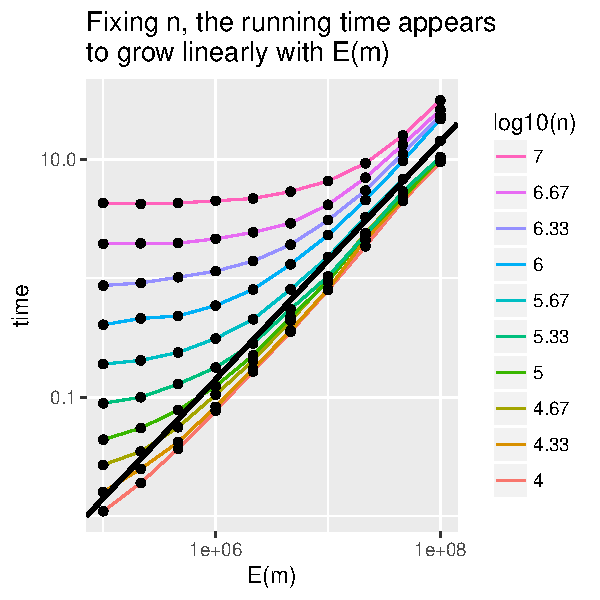
\includegraphics[width=7.2cm]{runTimeFixN.pdf}
    }
  \subfigure{
    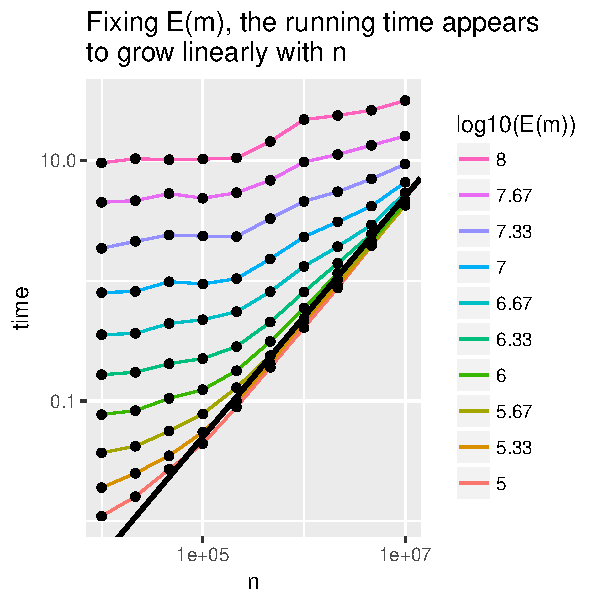
\includegraphics[width=7.2cm]{runTimeFixM.pdf}
    }
  \caption{Both plots present the same experimental data.  In the left plot, each  line corresponds to a different value of $n$ and they are presented as a function of $E(m)$.  In the right plot, each  line corresponds to a different value of $E(m)$ and they are presented as a function of $n$.  On the right side of both plots, the lines start to align with the solid black line, suggesting a linear dependence on $E(m)$ and $n$.  
  }
  %% label for entire figure
  \label{fig1}
\end{figure}
%To make it clearer, we do log-transformation for $time$ and $n$. In Figure \ref{speed1b}, the slope for the ``original" algorithm is approximately 2 and the slope for our ``fast" algorithm is approximately 1 which lends great credence to the fact that our ``fast" algorithm is $O(n)$ complexity while the original algorithm is $O(n^2)$ complexity.


%Figure \ref{Figure2} examines at what density (i.e. $m/n^2$) fRDGP and the element-wise technique have the same running time.  
%


\subsection{Comparison to a previous technique}

Previously, \cite{hagberg2015fast} studied a fast technique to generate sparse random kernel graphs.  Under the random kernel graph model, nodes $i$ and $j$ connect with probability $\kappa(i/n,j/n)$, where the  function $\kappa$ is non-negative, bounded, symmetric, measurable, and almost surely continuous.  This model class includes the SBM and the Degree-Corrected SBM.  It is difficult to see how a more general low rank model could be parameterized as a random kernel graph with an almost surely continuous $\kappa$.  For example, we suspect that Mixed Membership SBMs could not be parameterized as such.

The algorithm proposed in \cite{hagberg2015fast}  is fast when it is fast to compute  (i) the integral $F(y,a,b) = \int_a^b \kappa(x,y)dx$ and (ii) its roots, that is for any $y,a,r$, solve for $F(y,a,b) = r$.  Their software, which we  will refer to as  $fast$-$\kappa$ is in python and generates a NetworkX graph.  

For a simple benchmark to compare the running times of \texttt{fastRG} and $fast$-$\kappa$, Figure \ref{fig:compare} repeats the run  time experiment that  was  performed in \cite{hagberg2015fast}.  This simulation is for an Erd\H{o}s-R\'enyi graph with expected degree 10, for $n$ ranging between $5,000$ and $5M$.  Speed comparisons are troubled by the fact that our code returns an edge  list  in  \texttt{R} and $fast$-$\kappa$ returns a NetworkX graph  in  python. Converting from  an edge list to other data types takes longer than sampling the edge list with \texttt{fastRG}.  For example, converting the edge list to a sparse matrix (a type that is convenient for spectral estimators) takes about as long as  sampling the edge list with \texttt{fastRG}.  Converting the edge list to an igraph takes about 10x longer than sampling the edge list with \texttt{fastRG}.  There are three lines  in  Figure  \ref{fig:compare} for \texttt{fastRG}, one line for each data type (edge list, sparse adjacency matrix, and  igraph).  The speed comparison in Figure \ref{fig:compare} corresponds to the average running time over 10 simulations performed on a 2015 MacBook Pro, 2.8 GHz Intel Core i7, with  16 GB 1600 MHz DDR3  running Python 3.5.2  and \texttt{R} 3.3.2.  The slope of the  blue line  corresponds  to the running time $O(n \log  n)$.  
While none of these packages have been optimized for speed,  they are all sufficiently fast for  a wide  range  of purposes.  
%$fast$-$\kappa$ has the  advantage  of  sampling from a wider class of distributions. \texttt{fastRG} appears a bit faster.  


\begin{figure}[htbp] %  figure placement: here, top, bottom, or page
   \centering
   \textbf{Running time of \texttt{fastRG} and $fast$-$\kappa$ on Erd\H{o}s-R\'enyi graph with expected degree 10}
   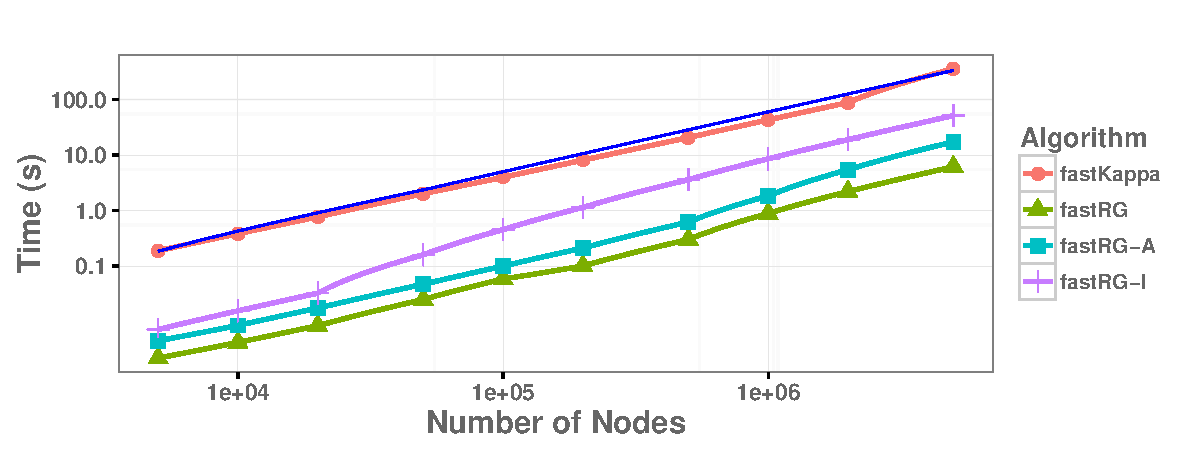
\includegraphics[width=6in]{compare.pdf} 
   \caption{As the  number of nodes increases (horizontal axis), all  of the running times increase in parallel to the solid blue line which gives the rate $O(n \log n)$.   The bottom three lines all correspond to \texttt{fastRG}, outputting three different graph types (edge list, sparse adjacency matrix, and igraph). For example,  in roughly  8 seconds, $fast$-$\kappa$ generates a graph with  20k nodes and \texttt{fastRG} generates an igraph with 1M nodes.  To  generate the random edge list on  1M nodes  with  \texttt{fastRG} takes less than 1 second}
   \label{fig:compare}
\end{figure}


\subsection{Simulating small and dense graphs with \texttt{fastRG}}

This section investigates the graph density at which \texttt{fastRG} becomes slower than simulating each element $A_{ij}$ as a Bernoulli random variable.  In Figure \ref{fig:dense}, the reported time to compute this naive (element-wise) algorithm includes both (i) the time it takes to compute the probabilities \texttt{eA = X\%*\%B\%*\%t(X)} and (ii) sample the edges \texttt{z = rbinom(length(eA), 1, eA)}.  The time for \\\texttt{fastRG} is for a directed graph, represented as a sparse matrix.  The time to compute \texttt{fastRG} also includes the time it takes to construct $X$ and $B$.   


Figure \ref{fig:dense} compares these two approaches on a set of Stochastic Blockmodels for values $K \in \{2, 5, 10\}$, $n \in \{500,1000,5000,10000\}$, and graph density $\rho = n^{-2} E(m)$ varying between $.02$ and $.35$.  In all simulations, the $S$ matrix is proportional to $I_K + J_K \in \mathds{R}^{K\times K}$, where $I_K$ is the identity matrix and $J_K$ is the matrix of ones.  The scale of $S$ is adjusted to ensure the correct density $\rho$.  For each model, both \texttt{fastRG} and the naive simulation are used to simulate two graphs.  The line is a quadratic fit with ordinary least squares. 
%\footnote{The \texttt{R} code for the dense approach, called \texttt{denseRG} in Figure \ref{fig:dense}, has two basic steps: (1) \texttt{eA = X\%*\%B\%*\%t(X)} and (2) \texttt{z = rbinom(length(eA), 1, eA)}.  We did not optimize this code.}     
In each panel, the vertical line is at $\rho = .25$, which is approximately the crossover point in all simulations.  For scale, $\rho = .25$ corresponds to expected degrees 125, 250, 1250, and 2,500 respectively for $n$ values $500,1000,5000,$ and $10000$.  


\begin{figure}[p] %  figure placement: here, top, bottom, or page
   \centering
   \textbf{Running time for small and dense graphs}
   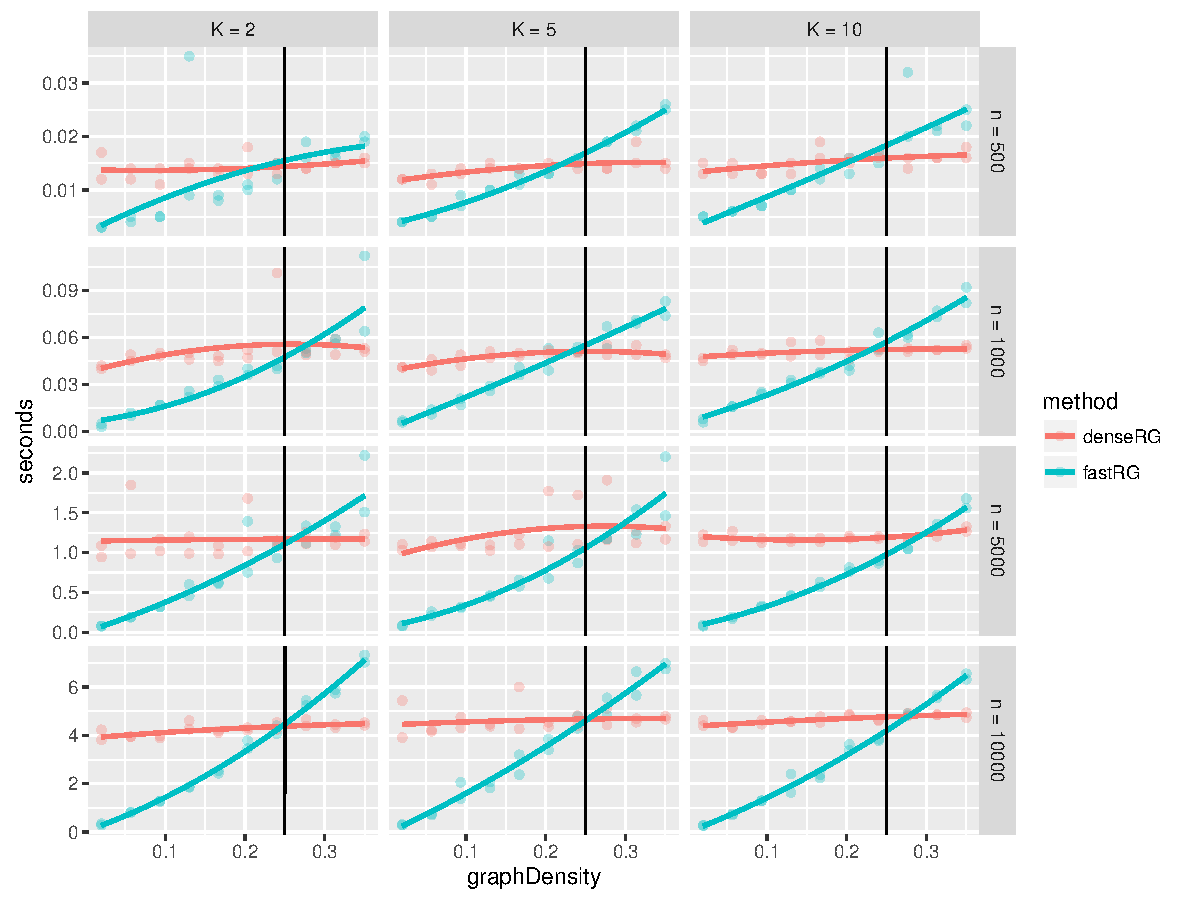
\includegraphics[width=6in]{denseRG.pdf} 
   \caption{This figure compares the run time of \texttt{fastRG} to the run time of simulating each $A_{ij}$  as a Bernoulli random variable (\texttt{denseRG} in the legend).  Note that the number of edges grows quadratically with the edge density.  So, as the density of the graph increases (horizontal axis), the running time of \texttt{fastRG} grows quadratically, whereas the running time of the naive algorithm does not depend on the density of the graph.  In this simulation, the crossover is around $\rho = .25$ (black line).  This figure shows that even for relatively small $n$ and in the dense regime,  \texttt{fastRG} has potential to be faster than the naive approach. }
   \label{fig:dense}
\end{figure}


%The SBM is a gRPG model where $X \in \{0,1\}^{n\times K}$ and there is a single one in each row.  If $X_{iu} = 1$, then the $i$th node belongs to block $u$. The elements of $S$ are in $[0,1]$ and $S_{uv}$ is the probability that a node in block $u$ connects to a node in block $v$.  The Degree-Corrected SBM is a Poisson gRPG with identity mean function.  Under this model, each row of $X\in \mathds{R}^{n \times K}$ has a single positive entry with all other entries equal to zero.  The Mixed Membership SBM is a Bernoulli gRPG with identity mean function.  Under this model, the rows of $X \in \mathds{R}^{n\times K}$ are non-negative. The Overlapping SBM is a Bernoulli gRPG with logistic mean function and the rows of $X \in \{0,1\}^{n \times K}$ are sparse.
%% and the Bernoulli edge probabilities are $\exp(\lambda_{ij}) / (1 + \exp(\lambda_{ij}))$.  


%The SBM is simulated as a gRPG with the identity link function.  This is possible by first transforming the matrix $S$; define $T_{uv} = -\\ln(1-S_{uv})$.  After thresholding a sample from \texttt{fastRG}$(X,T)$, it is a Bernoulli gRPG with link function $f(\lambda_{ij}) = 1- \exp(-\lambda_{ij})$. Under the SBM, each $\lambda_{ij}$ is an element of $T$.  So, $1- \exp(-T_{ij}) = S_{ij}$.  This implies that we can sample a Bernoulli SBM with $E(A) = XSX^T$ using \texttt{fastRG}$(X,T)$. For the other models, in general, there is no such transformation of $S$.  As a default, the code samples a Poisson gRPG with the identity link function. 

%The expected running time of this algorithm is $O(\|X\|_F^2 + nK)$, where $\|X\|_F^2$ is the expected number of edges.  However, in many settings, $X$

%Probabilistic inference has become a core technology in AI,
%largely due to developments in graph-theoretic methods for the 
%representation and manipulation of complex probability 
%distributions.  Whether in their guise as 
%directed graphs (Bayesian networks) or as undirected graphs (Markov 
%random fields), \emph{probabilistic graphical models} have a number 
%of virtues as representations of uncertainty and as inference engines.  
%Graphical models allow a separation between qualitative, structural
%aspects of uncertain knowledge and the quantitative, parametric aspects 
%of uncertainty...\\
%
%{\noindent \em Remainder omitted in this sample. See http://www.jmlr.org/papers/ for full paper.}
%
%% Acknowledgements should go at the end, before appendices and references
%
%\newpage
\acks{This research was supported by NSF grant DMS-1612456 and ARO grant W911NF-15-1-0423.}
%from the National Science Foundation (NSF grant IIS-9988642)
%and the Multidisciplinary Research Program of the Department
%of Defense (MURI N00014-00-1-0637). }

% Manual newpage inserted to improve layout of sample file - not
% needed in general before appendices/bibliography.

%\newpage
\appendix
  \renewcommand{\appendixname}{Appendix~\Alph{section}}

\section{Proofs}
For an integer $d$, define $1_d \in \mathds{R}^d$ as a vector of ones.  The proof of Theorem \ref{theoremRDPG} requires the following lemma, which says that a vector (or matrix) of independent Poisson entries becomes multinomial when you condition on the sum of the vector (or matrix).
\begin{lemma}
\label{lemma1}
Let $A \in \mathds{R}^{n \times n}$ be the random matrix whose $i,j th$ element $A_{ij} \overset{i.d.}{\sim}$ Pois$(\lambda_{ij})$ $i,j=1, \ \dots, \ n$.
Then conditioned on $\sum_{i,j}A_{ij} =  1_n^TA1_n=m$,
\begin{equation*}
(A_{11},\ A_{12},\ \dots,\ A_{nn}) \sim Multinomial(m,\ \lambda / \sum_{ij} \lambda_{ij})
\end{equation*}
where $\lambda = (\lambda_{11},\ \lambda_{12},\ \dots,\ \lambda_{nn})$.  That is, let $a\in \mathds{R}^{n \times n}$ be a fixed matrix of integers with $1_n^Ta1_n=m$, then
\begin{eqnarray*}
\mathbb{P}(A = a|1_n^T A 1_n = m)&=&\mathbb{P}(A_{11} = a_{11}, \ A_{12} = a_{12},\ \dots,\ A_{nn} = a_{nn}|1_n^T A 1_n = m) \\
&=&  \frac{m!}{\prod_{i,j}a_{ij}!} \prod_{i,j} \left(\frac{\lambda_{ij}}{\lambda_{11} + \lambda_{12}+\cdots +\lambda_{nn}} \right)^{a_{ij}}.
\end{eqnarray*}
\end{lemma}

\vspace{.2 in}

For completeness, a proof of this classical result is given at the end of the paper. The next proof is a proof of Theorem \ref{theoremRDPG}.

\vspace{.2 in}

%The next Lemma shows that the edges XXX
%Why do we need this lemma?
 %\begin{lemma}
%\label{lemma2}
%We use the same notations as Lemma \ref{lemma1}. In Lemma \ref{lemma1}, define the orders of the sampled $m$ units as $L_1$, $L_2$, \dots, $L_m$, taking values in $\{11,\ 12,\ \dots,\ nn\}$. We have $A_{ij} = \sum_{t=1}^m \mathds{1}(L_t = ij)$ and for all k,
%\[\mathbb{P}(L_k = l_k | L_1=l_1,\ \dots,\  L_{k-1}=l_{k-1}) = \mathbb{P}(L_k = l_k)\]
%\end{lemma}
%\begin{proof}[proof of Lemma 2]
%If $L_1=l_1,\ \dots,\  L_k=l_k$, then denote $b_{ij} = \sum_{t=1}^k \mathds{1}(l_t = ij)$. We have
%\begin{align*}
%\mathbb{P}(L_1=l_1,\ \dots,\  L_k=l_k)&=(\frac{k!}{\prod_{i,j}b_{ij}!})^{-1}\mathbb{P}(A_{11} = b_{11},\  A_{12}=b_{12},\ \dots,\ A_{nn} = b_{nn}) \\
%&=(\frac{k!}{\prod_{i,j}{b_{ij}!}})^{-1}\frac{k!}{\prod_{i,j}b_{ij}!} \prod_{i,j} \left(\frac{\lambda_{ij}}{\lambda_{11} + \lambda_{12}+\dots +\lambda_{nn}} \right)^{b_{ij}}\\
%&=\prod_{i,j} \left(\frac{\lambda_{ij}}{\lambda_{11} + \lambda_{12}+\dots +\lambda_{nn}} \right)^{b_{ij}}
%\end{align*}
%Denote $A_{11} = a_{11}$, $A_{12} = a_{12}$, \dots, $A_{nn}$ = $a_{nn}$ as the temporary result $L_1=l_1$, \dots, $L_{k-1}$=$l_{k-1}$ gives.
%\begin{align*}
%\mathbb{P}(L_k = l_k | L_1=l_1,\ \dots, \ L_{k-1}=l_{k-1})&=
%\frac{\left(\frac{\lambda_{l_k}}{\lambda_{11} + \lambda_{12}+\cdots +\lambda_{nn}} \right)^{a_{l_k}+1}\prod_{ij\ne l_k} \left(\frac{\lambda_{l_k}}{\lambda_{11} + \lambda_{12} +\cdots +\lambda_{nn}} \right)^{a_{ij}}}
%{\sum_{i,j}^n \left(\frac{\lambda_{l_k}}{\lambda_{11} + \lambda_{12}+\cdots +\lambda_{nn}} \right)^{a_{ij}+1}\prod_{pq\ne ij} \left(\frac{\lambda_{l_k}}{\lambda_{11} + \lambda_{12}+\cdots +\lambda_{nn}} \right)^{a_{pq}}}\\
%&=\frac{ \left(\frac{\lambda_{l_k}}{\lambda_{11} + \lambda_{12}+\cdots +\lambda_{nn}} \right)}
%{\sum_{i,j}^n\left(\frac{\lambda_{l_k}}{\lambda_{11} + \lambda_{12}+\cdots +\lambda_{nn}} \right)}\\
%&=\frac{\lambda_{l_{k}}}{\sum_{i,j}^n\lambda_{ij}}
%\end{align*}
%\end{proof}



\begin{proof}
Let $A$ come from the Poisson gRPG with $X$ and $S$ and identity mean function.  Let $\tilde A$ be a sample from \texttt{fastRG}.   For any fixed adjacency matrix $a$, we will show that $\mathbb{P}(A = a)=\mathbb{P}(\tilde A = a)$.

Define $m = 1_n^Ta1_n$ and decompose the probabilities,
\begin{eqnarray}
\mathbb{P}(A = a) &=& \mathbb{P}(1_n^T A 1_n =m) \mathbb{P}(A=a| 1_n^T A 1_n =m) \\
\mathbb{P}(\tilde A = a) &=& \mathbb{P}(1_n^T \tilde A 1_n =m) \mathbb{P}(\tilde A=a| 1_n^T \tilde A 1_n =m).
\end{eqnarray}
The proof will be divided into two parts.  The first part shows that $\mathbb{P}(1_n^T A 1_n =m) = \mathbb{P}(1_n^T \tilde A 1_n =m)$ and the second part will show that  $\mathbb{P}(A=a| 1_n^T A 1_n =m) = \mathbb{P}(\tilde A=a| 1_n^T \tilde A 1_n =m)$.

\textbf{Part 1:} 
%Note that $A_{ij} \overset{i.d.}{\sim} Poisson(\lambda_{ij})$. 
The sum of independent Poisson variables is still Poisson, 
\[\sum_{ij} A_{ij} \sim Poisson(\sum_{ij}\lambda_{ij}).\]  
So, we must only show that $1_n^T A 1_n$ and $1_n^T \tilde A 1_n$ have the same Poisson parameter:
%to show that $\mathbb{P}(1_n^T A 1_n =m) = \mathbb{P}(1_n^T \tilde A 1_n =m)$, 
%we must only show that $\sum_{ij}\lambda_{ij} = \sum_{uv} \tilde S_{uv}$,
\[\sum_{ij}\lambda_{ij} = 1_n^T X S X 1_n  =  1_n^T XC C^{-1} S C^{-1} C X 1_n  =  1_n^T \tilde X\tilde S \tilde X 1_n  =  1_n^T \tilde X\tilde S \tilde X 1_n  =  1_K^T \tilde S 1_K  =  \sum_{u,v} \tilde S_{uv}.\]

%\begin{eqnarray*}
%\sum_{ij}\lambda_{ij} &=& 1_n^T X S X 1_n \\
%&=& 1_n^T XC C^{-1} S C^{-1} C X 1_n \\
%&=& 1_n^T \tilde X\tilde S \tilde X 1_n \\
%&=& 1_n^T \tilde X\tilde S \tilde X 1_n \\
%&=& 1_K^T \tilde S 1_K \\
%&=& \sum_{u,v} \tilde S_{uv}
%\end{eqnarray*}



\textbf{Part 2:} After conditioning on $1_n^T A 1_n = m$,  Lemma \ref{lemma1} shows that $A$ has the multinomial distribution.  In \texttt{fastRG}, we first sample $1_n^T \tilde A1_n$ and then add edges with the multinomial distribution.  So,  we must only show that the multinomial edge probabilities are equal for $A$ and $\tilde A$.  From Lemma \ref{lemma1}, the multinomial edge probabilities for $A$ are $\lambda_{ij} /\sum_{a,b} \lambda_{ab} $.
%\begin{eqnarray}
%
%\end{eqnarray}
%To compute the multinomial edge probabilities, condition on $\sum_{i,j}A_{ij}= 1$.   To compute the edge probability for element $i,j$, denote $\mathds{1}_{ij}$ as a matrix which has a $1$ at $ij$ th position, and $0$s otherwise.
%\begin{eqnarray}
%\nonumber \mathbb{P}(A = \mathds{1}_{ij} | m = 1  )
%%                            &=& \frac{1!}{\prod_{a,b}A_{ab}!} \prod_{a,b} \left(\frac{\lambda_{ab}}{\lambda_{11} + \lambda_{12} + \dots +\lambda_{nn}} \right)^{A_{ab}}\\
%\nonumber                             &=& \frac1{(0!)^{n^2-1}\cdot1!}\cdot\frac{\lambda_{ij}}{\sum_{a,b} \lambda_{ab}}\\
%\label{eq:oneedge}                            &=& \frac{\langle x_i, x_j\rangle_S}{\sum_{a,b} \langle x_a, x_b\rangle_S}.
%\end{eqnarray}
To compute the multinomial edge probabilities for $\tilde A$, recall that $(I,J)$ is a single edge added to the graph in \texttt{fastRG}. By Theorem \ref{theorem:xlr},
\[\mathbb{P}(\tilde A_{ij} = 1 | 1_n^T\tilde A1_n = 1  ) =  \mathbb{P}\big((I,J)=(i,j)\big) = \frac{\langle x_i, x_j\rangle_S}{\sum_{a,b} \langle x_a, x_b\rangle_S} =  \frac{\lambda_{ij}}{\sum_{a,b} \lambda_{ab}}\]
%\begin{eqnarray*}
%\mathbb{P}(\tilde A_{ij} = 1 | 1_n^T\tilde A1_n = 1  ) &=& \mathbb{P}\big((I,J)=(i,j)\big) \\
%&=& \sum_{u,v} \mathbb{P}(I=i,J=j|U=u, V=v)\mathbb{P}(U=u, V=v)\\
%                            &=& \sum_{u,v} \tilde X_{iu} \tilde X_{ju} \frac{\tilde S_{uv}}{\sum_{u,v} \tilde S_{u,v}}\\
%                            &=& \frac{ \sum_{u,v} X_{iu} X_{ju} S_{uv}}{\sum_{u,v} \tilde S_{u,v}}\\
%                            &=& \frac{\langle x_i, x_j\rangle_S}{\sum_{a,b} \langle x_a, x_b\rangle_S}.\\
%                            &=& \frac{\lambda_{ij}}{\sum_{a,b} \lambda_{ab}}. 
%%                            &= \sum_u \frac{X_{iu}X_{ju}}{(\sum_t X_{tu})^2}\cdot\\
%%                            \frac{(\sum_t X_{tu})^2}{\sum_{a,b} \langle x_a, x_b\rangle}\\
%%                            &= \frac{\langle x_i, x_j\rangle}{\sum_{a,b} \langle x_a, x_b\rangle}.
%\end{eqnarray*}
This concludes the proof.
\end{proof}

%\begin{remark}
%If one wishes to have a symmetric graph, then there are a few trivial changes to make in the argument.  First, in Lemma \ref{lemma1}, only consider $A_{ij}$ for $i\le j$.  
%
% record the edges of \texttt{fastRG} as $\{I,J\}$ instead of $(I, J)$.  
%\end{remark}
%For a graph without any self-loop, Equation \eqref{eq:oneedge} becomes
%\begin{align*}
%\mathbb{P}(A = \mathds{1}_{ij} | m = 1  )
%                            &= \frac{\langle x_i, x_j\rangle_S}{\sum_{a\neq b} \langle x_a, x_b\rangle_S}.\\
%\end{align*}
%
%
%
%
%XXXX  Why do we need this argument?  we don't need to keep resampling these edges because the diagonal should no longer go into the computation of $m$ ... that is where the gap in the proof is.. right? XXXX
%\begin{remark}\label{remark:selfloopproof}
%Then we can deal with graphs without any self-loop. We still denote $(I,J)$ as a single edge added in the algorithm. To get one edge $(I,J)$ with $I\neq J$, we need to sample $Y$ times in algorithm 1 and $Y$ is geometric distribution with success probability $p=\mathbb{P}(I\neq J)$. Then for $i \neq j$,
%
%XXXX Can you check that this still holds.... XXXX
% \begin{align*}
%\mathbb{P}\big((I,J)=(i,j)\big)
%    &= \sum_{k=1}^\infty \mathbb{P}(I=J)^{k-1} \cdot \mathbb{P}\big((I,J)=(i,j)\big)\\
%    &= \big(1-\mathbb{P}(I=J)\big)^{-1} \cdot \mathbb{P}\big((I,J)=(i,j)\big)\\
%    &= \big(1 - \sum_{h=1}^n\frac{\langle x_h, x_h\rangle}{\sum_{a,b} \langle x_a, x_b\rangle}\big)^{-1} \cdot
%                            \frac{\langle x_i, x_j\rangle}{\sum_{a,b} \langle x_a, x_b\rangle}\\
%    &= \big(\frac{\sum_{a\ne b}\langle x_a, x_b\rangle}{\sum_{a,b}\langle x_a, x_b\rangle}\big)^{-1} \cdot
%                            \frac{\langle x_i, x_j\rangle}{\sum_{a,b} \langle x_a, x_b\rangle}\\
%    &= \frac{\langle x_i, x_j\rangle}{\sum_{a\ne b} \langle x_a, x_b\rangle}
%\end{align*}
%\end{remark}
%
%


%\section{}

\begin{proof}[Proof of Theorem \ref{theoremThresh}]
%Let $U_{ij} \overset{i.i.d}{\sim}$ $Uniform(0,1)$. Define $t(\tilde A)$ and $B$: 
%\begin{align*}
%t(\tilde A)_{ij} &= \bold{1}(U_{ij}>1-e^{-\lambda_{ij}}),\\
%B_{ij} &= \bold{1}(U_{ij}>\lambda_{ij}).
%\end{align*}
%Note that $t(\tilde A)$ and $B$ have the correct distribution.  By Taylor expansion,
%%To calculate  $E\|t(\tilde A) - B\|^2_F$ and $E\|B\|^2_F$:
%\begin{eqnarray*}
%E\|t(\tilde A) - B\|^2_F &=& \sum_{i,j}(\lambda_{ij}-(1-e^{-\lambda_{ij}}))\\
%&=& \sum_{i,j} \sum_{k=2}^\infty (-\lambda_{ij})^k/k!\\
%&=& \sum_{i,j} O(\lambda_{ij}^2)\\
%&=& \sum_{i,j} O((\alpha_n/n)^2)\\
%&=& O(\alpha_n^2).
%\end{eqnarray*}
%At the same time, $E\|B\|_F^2  = \sum_{ij} \lambda_{ij} > c \alpha_n n $.  So, define $\tilde A$ 
%\begin{proof}
Let $U_{ij} \overset{i.i.d}{\sim}$ $Uniform(0,1)$. Define $\mathcal{A}$ and $\mathcal{B}$: 
\begin{align*}
\mathcal{A}_{ij} &= \bold{1}(U_{ij}>1-e^{-\lambda_{ij}}),\\
\mathcal{B}_{ij} &= \bold{1}(U_{ij}>\lambda_{ij}).
\end{align*}
Note that $\mathcal{A}$ and $\mathcal{B}$ are equal in distribution to $ t(\tilde A)$ and $B$ respectively.  By Taylor expansion,
\[E\|\mathcal{A} - \mathcal{B}\|^2_F = \sum_{i,j}(\lambda_{ij}-(1-e^{-\lambda_{ij}})) =  \sum_{i,j} \sum_{k=2}^\infty (-\lambda_{ij})^k/k! =  \sum_{i,j} O(\lambda_{ij}^2) =  \sum_{i,j} O((\alpha_n/n)^2) =  O(\alpha_n^2).\]
%%To calculate  $E\|\mathcal{A} - \mathcal{B}\|^2_F$ and $E\|\mathcal{B}\|^2_F$:
%\begin{eqnarray*}
%E\|\mathcal{A} - \mathcal{B}\|^2_F &=& \sum_{i,j}(\lambda_{ij}-(1-e^{-\lambda_{ij}}))\\
%&=& \sum_{i,j} \sum_{k=2}^\infty (-\lambda_{ij})^k/k!\\
%&=& \sum_{i,j} O(\lambda_{ij}^2)\\
%&=& \sum_{i,j} O((\alpha_n/n)^2)\\
%&=& O(\alpha_n^2).
%\end{eqnarray*}
Then, $E\|B\|_F^2  = \sum_{ij} \lambda_{ij} > c \alpha_n n $.  So, defining $t(\tilde A)$ and $B$ with the above coupling yields the result.
%\[\frac{E\|\mathcal{A} - \mathcal{B}\|^2_F}{E\|\mathcal{B}\|^2_F}  = O(\alpha_n/n).\]
%\[\frac{E\|t(\tilde A) - B\|^2_F}{E\|B\|^2_F}  = O(\alpha_n/n).\]

\end{proof}

%\appendix
%\section*{Appendix A.}
%\label{app:theorem}
%
%% Note: in this sample, the section number is hard-coded in. Following
%% proper LaTeX conventions, it should properly be coded as a reference:
%
%%In this appendix we prove the following theorem from
%%Section~\ref{sec:textree-generalization}:
%
%In this appendix we prove the following theorem from
%Section~6.2:
%
%\noindent
%{\bf Theorem} {\it Let $u,v,w$ be discrete variables such that $v, w$ do
%not co-occur with $u$ (i.e., $u\neq0\;\Rightarrow \;v=w=0$ in a given
%dataset $\dataset$). Let $N_{v0},N_{w0}$ be the number of data points for
%which $v=0, w=0$ respectively, and let $I_{uv},I_{uw}$ be the
%respective empirical mutual information values based on the sample
%$\dataset$. Then
%\[
%	N_{v0} \;>\; N_{w0}\;\;\Rightarrow\;\;I_{uv} \;\leq\;I_{uw}
%\]
%with equality only if $u$ is identically 0.} \hfill\BlackBox
%
%\noindent
%{\bf Proof}. We use the notation:
%\[
%P_v(i) \;=\;\frac{N_v^i}{N},\;\;\;i \neq 0;\;\;\;
%P_{v0}\;\equiv\;P_v(0)\; = \;1 - \sum_{i\neq 0}P_v(i).
%\]
%These values represent the (empirical) probabilities of $v$
%taking value $i\neq 0$ and 0 respectively.  Entropies will be denoted
%by $H$. We aim to show that $\fracpartial{I_{uv}}{P_{v0}} < 0$....\\
%
%{\noindent \em Remainder omitted in this sample. See http://www.jmlr.org/papers/ for full paper.}

\begin{proof}[proof of Lemma 1]
\begin{align*}
\mathbb{P}(A=a|1_n^T A 1_n = m) &= \frac{\mathbb{P}(A=a)}{\mathbb{P}(1_n^T A 1_n = m)}
 = \dfrac{\prod_{i,j} \dfrac{\lambda_{ij}^{a_{ij}}}{a_{ij}!}e^{-\lambda_{ij}}}{\dfrac{(\lambda_{11} + \lambda_{12}+\cdots +\lambda_{nn})^m}{m!}e^{-({\lambda_{11} + \lambda_{12}+\cdots +\lambda_{nn})}}}\\
& = \frac{m!}{\prod_{i,j}a_{ij}!} \prod_{i,j} \left(\frac{\lambda_{ij}}{\lambda_{11} + \lambda_{12}+\cdots +\lambda_{nn}} \right)^{a_{ij}}
\end{align*}
\end{proof}


\vskip 0.2in
%\bibliography{bibfile}


\begin{thebibliography}{13}
\providecommand{\natexlab}[1]{#1}
\providecommand{\url}[1]{\texttt{#1}}
\expandafter\ifx\csname urlstyle\endcsname\relax
  \providecommand{\doi}[1]{doi: #1}\else
  \providecommand{\doi}{doi: \begingroup \urlstyle{rm}\Url}\fi

\bibitem[Airoldi et~al.(2008)Airoldi, Blei, Fienberg, and
  Xing]{Airoldi2008Mixed}
E Airoldi, E Blei, S Fienberg, and E Xing.
\newblock Mixed membership stochastic blockmodels.
\newblock \emph{Journal of Machine Learning Research}, 9\penalty0 (5):\penalty0
  1981--2014, 2008.

\bibitem[Cai et~al.(2016)Cai, Campbell, and Broderick]{cai2016edge}
D Cai, T Campbell, and T Broderick.
\newblock Edge-exchangeable graphs and sparsity.
\newblock In \emph{Advances in Neural Information Processing Systems}, pages
  4242--4250, 2016.

\bibitem[Crane and Dempsey(2016)]{crane2016edge}
H Crane and W Dempsey.
\newblock Edge exchangeable models for network data.
\newblock \emph{arXiv preprint arXiv:1603.04571}, 2016.

\bibitem[Hagberg and Lemons(2015)]{hagberg2015fast}
A Hagberg and N Lemons.
\newblock Fast generation of sparse random kernel graphs.
\newblock \emph{PloS one}, 10\penalty0 (9):\penalty0 e0135177, 2015.

\bibitem[Herlau et~al.(2016)Herlau, Schmidt, and M\o~rup]{NIPS2016_6521}
T Herlau, M Schmidt, and M M\o~rup.
\newblock Completely random measures for modelling block-structured sparse
  networks.
\newblock In \emph{Advances in Neural Information Processing Systems 29}. 2016.

\bibitem[Holland et~al.(1983)Holland, Laskey, and
  Leinhardt]{Holland1983Stochastic}
P Holland, K Laskey, and S Leinhardt.
\newblock Stochastic blockmodels: First steps.
\newblock \emph{Social Networks}, 5\penalty0 (2):\penalty0 109--137, 1983.

\bibitem[Karrer and Newman(2011)]{PhysRevE.83.016107}
B Karrer and M Newman.
\newblock Stochastic blockmodels and community structure in networks.
\newblock \emph{Phys. Rev. E}, 83:\penalty0 016107, Jan 2011.

\bibitem[Latouche and Ambroise(2011)]{Latouche2011Overlapping}
P Latouche and C Ambroise.
\newblock Overlapping stochastic block models with application to the french
  political blogosphere.
\newblock \emph{Annals of Applied Statistics}, 5\penalty0 (1):\penalty0
  309--336, 2011.

\bibitem[Lehoucq et~al.(1995)Lehoucq, Sorensen, and Vu]{lehoucqarpack}
R Lehoucq, D Sorensen, and P Vu.
\newblock Arpack: An implementation of the implicitly re-started arnoldi
  iteration that computes some of the eigenvalues and eigenvectors of a large
  sparse matrix.
\newblock \emph{Available from netlib@ ornl. gov under the directory
  scalapack}, 1995.

\bibitem[{Todeschini} and {Caron}(2016)]{2016arXiv160202114T}
A {Todeschini} and F {Caron}.
\newblock {Exchangeable Random Measures for Sparse and Modular Graphs with
  Overlapping Communities}.
\newblock \emph{arXiv preprint arXiv:1602.02114}, February 2016.

\bibitem[Vose(1991)]{vose1991linear}
M Vose.
\newblock A linear algorithm for generating random numbers with a given
  distribution.
\newblock \emph{IEEE Transactions on software engineering}, 17\penalty0
  (9):\penalty0 972--975, 1991.

\bibitem[Walker(1977)]{walker1977efficient}
A  Walker.
\newblock An efficient method for generating discrete random variables with
  general distributions.
\newblock \emph{ACM Transactions on Mathematical Software}, 3\penalty0
  (3):\penalty0 253--256, 1977.

\bibitem[Young and Scheinerman(2007)]{Young2007}
S  Young and E  Scheinerman.
\newblock \emph{Random Dot Product Graph Models for Social Networks}, pages
  138--149.
\newblock Springer Berlin Heidelberg, Berlin, Heidelberg, 2007.

\end{thebibliography}



\end{document}
